%-  LaTeX source file

%-  performance.tex ~~
%
%   This is the fourth section of the paper.
%
%                                                   ~~ last updated 29 Oct 2018

This section contains almost all of the quantitative results of this paper.

%The CSC108 project operates under the assumption that the constraints imposed
%on its jobs by OLCF prevent it from competing for resources with other
%projects. In order to assess the effectiveness of this strategy, we have
%pursued several lines of inquiry by sampling data from the MOAB scheduler on
%Titan.
%
%Availability note: code supporting this section is available at
%\url{https://github.com/ATLAS-Titan/moab-data}. 


Characterizing the performance of PanDA on Titan presents a number of
challenges, thanks especially to the facts that PanDA utilizes its resources
both directly and opportunistically and also that Titan has many users who are
running production workloads of their own. Thus, this section investigates two
areas: showing that PanDA was successfully ported and scaled on Titan, and
assessing the impact of PanDA on the other projects and users of Titan.

Note that the project name ``CSC108'' represents the official name of this
project on Titan, and all of the jobs of CSC108 run in so-called ``backfill
mode.'' (MAKE SURE THIS IS EXPLAINED SOMEWHERE ELSE IN THE PAPER, OR ELSE
EXPLAIN IT HERE.) There are two other identifiers for PanDA projects on Titan,
which are ``HEP110'' and ``HEP113''. HEP110 and HEP113 use resources on Titan
directly through an ALCC allocation.

%\subsubsection{Blocking Probability}
%\label{subsubsec:blockingprobability}
%
%We begin with a simple model that defines an event called a ``block'' and then
%detects its occurrences within the data.
%
%Let $C_i$ be the abstract resources in use by CSC108 at the $i^{\text{th}}$
%sample point in time, and let $U_i$ be the unused (idle) resources remaining on
%Titan. We then define a boolean $B_i$ representing a ``block'' to be 1 if there
%exists at least one job at the $i^{\text{th}}$ sample point which requests
%$(C_i + U_i)$ resources or less, and we define $B_i$ to be zero otherwise.
%
%Summing $B_i$ over all $i$ gives a count of sample points at which a block
%occurred, and dividing that count by the number of total sample points yields a
%quantity we will term a ``blocking fraction''.
%
%To use this model for our concrete data set, we define the resources in
%question to be requested processors (or requested nodes).
%
%(Specific numbers and graphs go here.)

\subsection{Scaling PanDA on Titan}
\label{subsec:scaling}

(This section should have lots of the kinds of plots that Danila always shows
and that Sean always puts on his posters, like Titan core hours by month and
stuff like that \ldots see Figure~\ref{fig:time-vs-nodes}.)

% For two-column wide figures use
\begin{figure*}
% Use the relevant command to insert your figure file.
% For example, with the graphicx package use
  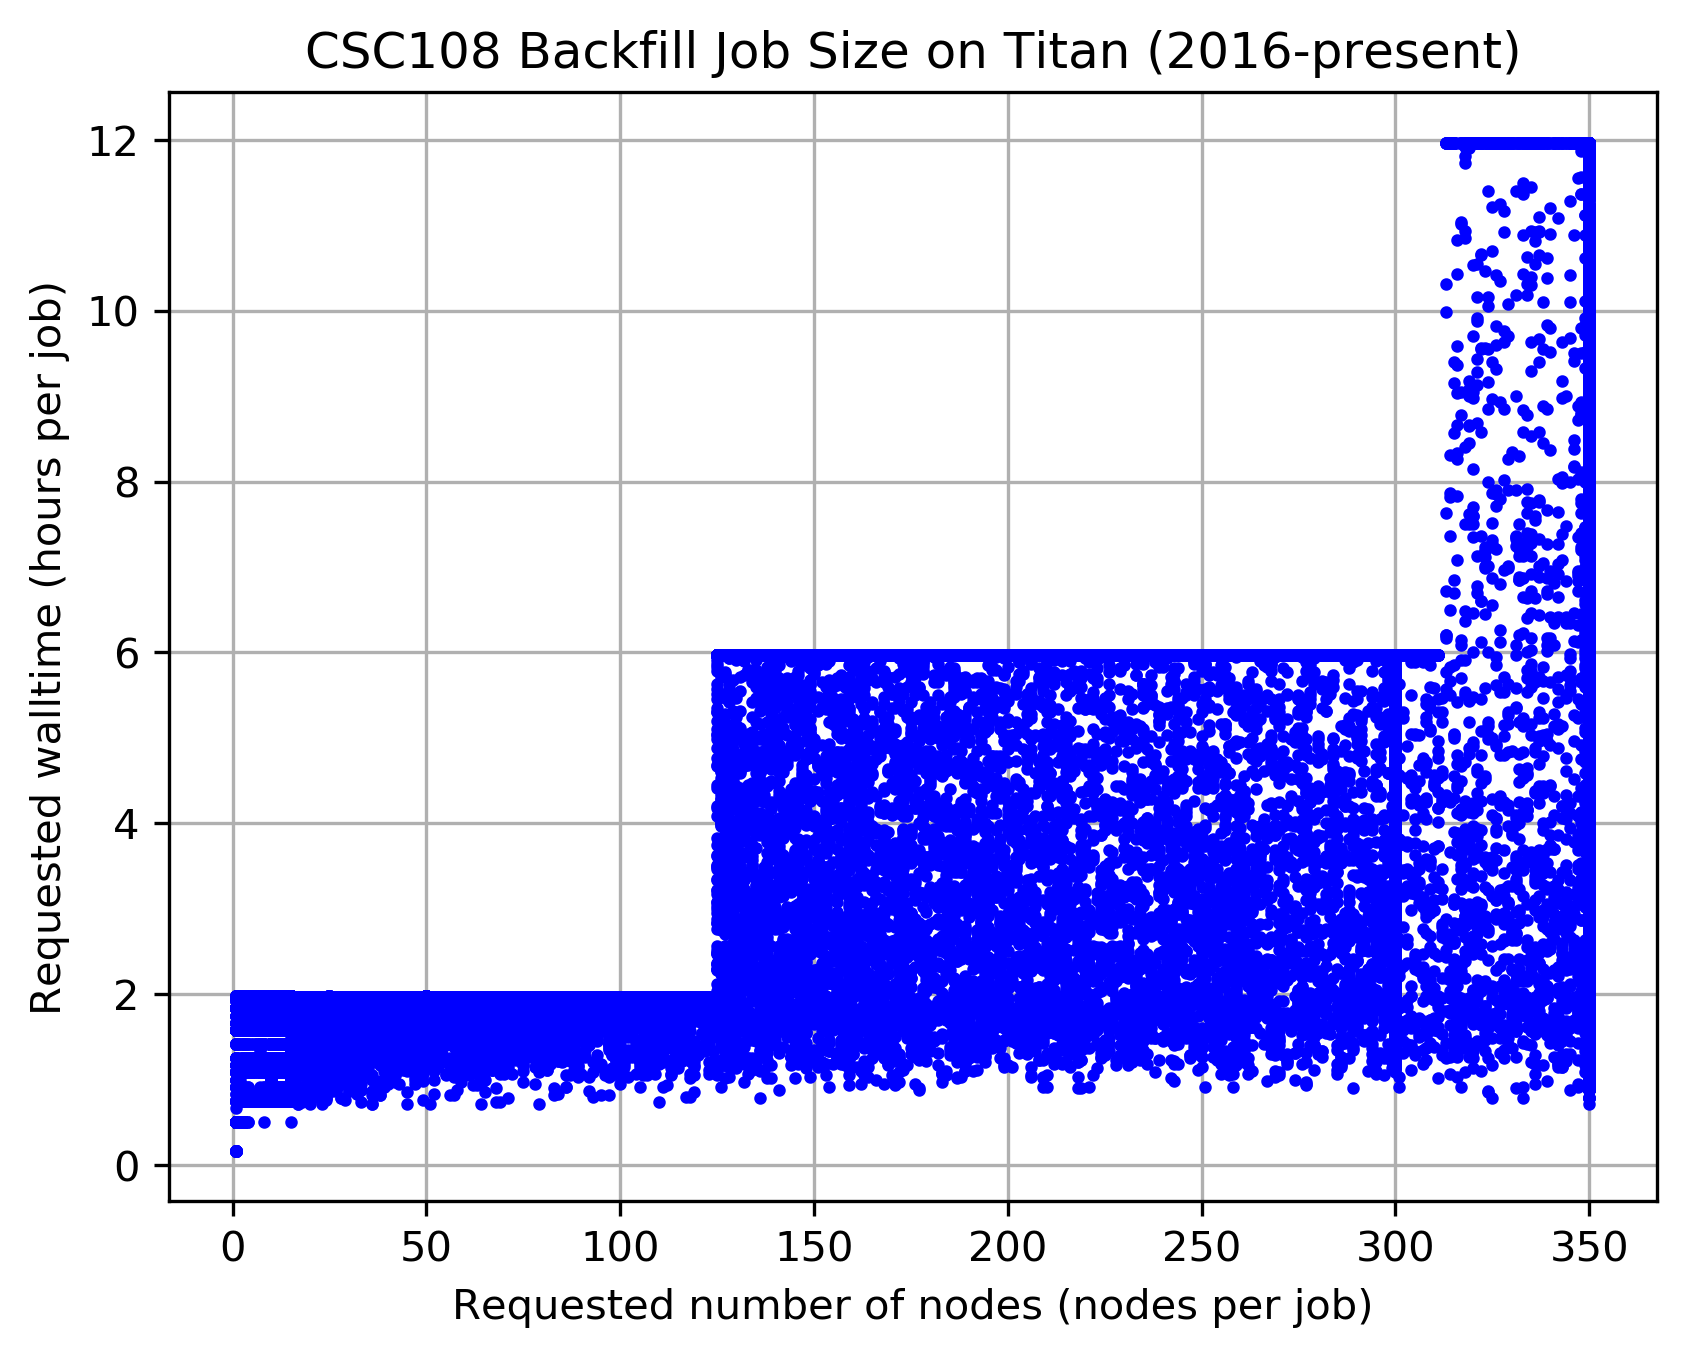
\includegraphics[width=0.75\textwidth]{images/time-vs-nodes-backfill.png}
% figure caption is below the figure
\caption{This figure shows that the PanDA deployment on Titan runs CSC108 jobs
that vary in size by time and by space. The stair steps occur due to the
constraints from Titan policy by bin. The jobs in the bottom left ``column''
run in bin 5, the jobs in the middle are running in bin 4, and the jobs on the
right are bin 3. Note that the rightmost boundary of the plot, at 350 nodes,
represents a self-imposed constraint.}
\label{fig:time-vs-nodes}
\end{figure*}






\subsection{Impact of PanDA on Titan}
\label{subsec:impact}

Having shown that PanDA has indeed ported and scaled successfully on Titan, we
now investigate the impact of PanDA on Titan, especially on its other users
and their projects and workloads. To this end, we pursue three main routes,
which are to assess PanDA's impact on wait times (TQ), throughput, and
utilization on Titan.




\subsubsection{WaitTimes}
\label{subsubsec:waittimes}

Lorem ipsum \ldots






\subsubsection{Throughput}
\label{subsubsec:throughput}

Lorem ipsum \ldots


% For two-column wide figures use
\begin{figure*}
% Use the relevant command to insert your figure file.
% For example, with the graphicx package use
  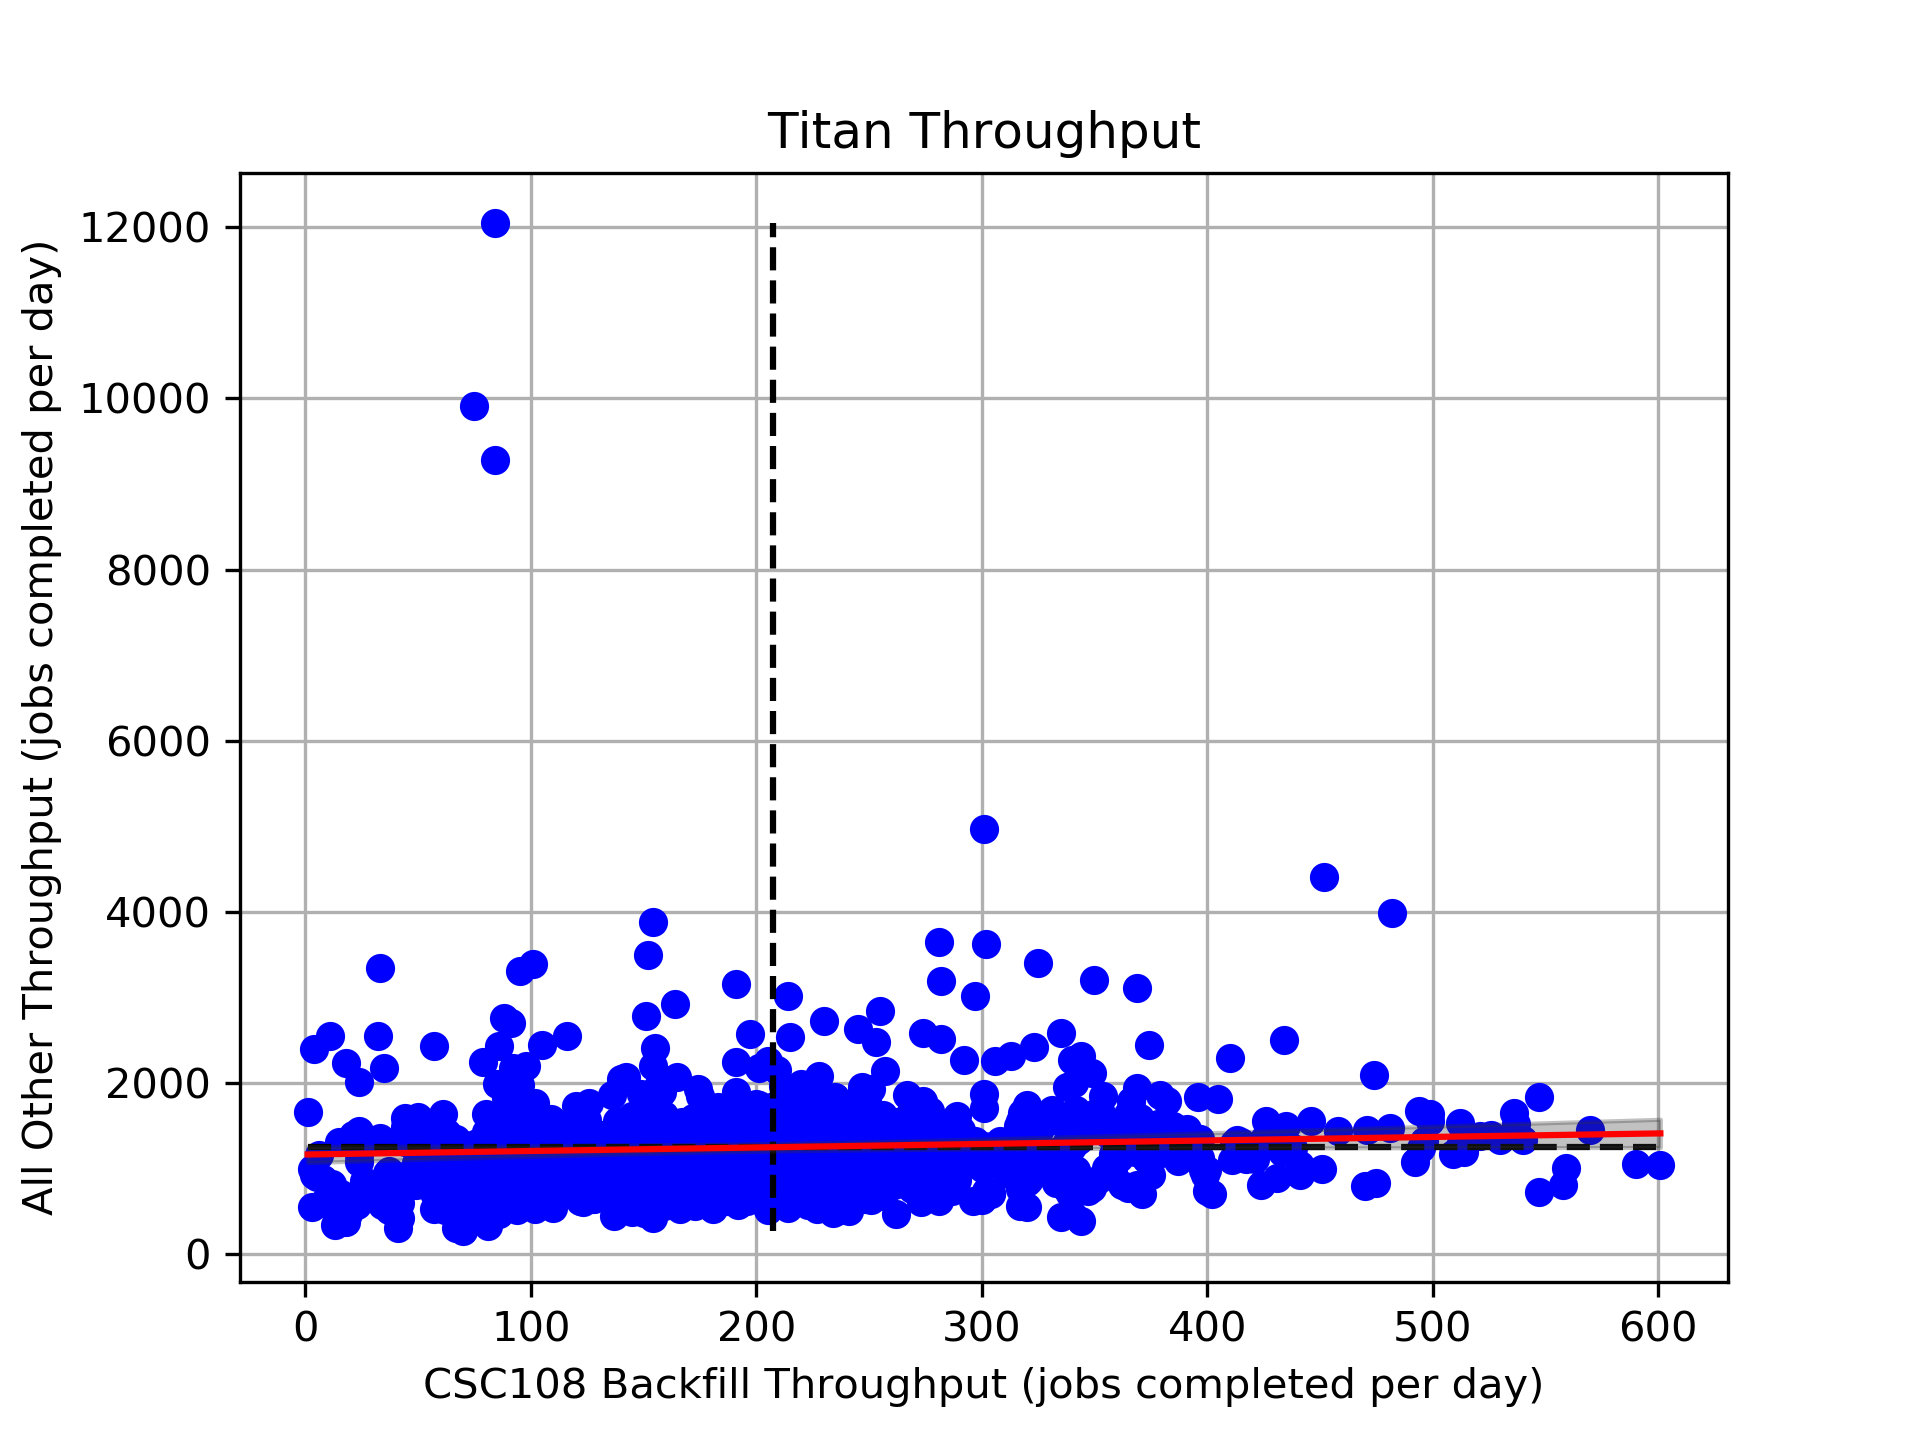
\includegraphics[width=0.75\textwidth]{images/linfit-throughput-all.png}
% figure caption is below the figure
\caption{This figure shows the relationship between CSC108 backfill throughput
and overall throughput by counting jobs completed by day.}
\label{fig:throughput-all}
\end{figure*}




\subsubsection{Utilization}
\label{subsubsec:utilization}

Lorem ipsum \ldots





%-  vim:set syntax=tex:
